% Use only LaTeX2e, calling the article.cls class and 12-point type.

\documentclass[12pt]{article}

% Users of the {thebibliography} environment or BibTeX should use the
% scicite.sty package, downloadable from *Science* at
% www.sciencemag.org/about/authors/prep/TeX_help/ .
% This package should properly format in-text
% reference calls and reference-list numbers.

\usepackage{scicite}

% Use times if you have the font installed; otherwise, comment out the
% following line.

\usepackage{times}

\usepackage{graphicx}

\usepackage{lscape }

% The preamble here sets up a lot of new/revised commands and
% environments.  It's annoying, but please do *not* try to strip these
% out into a separate .sty file (which could lead to the loss of some
% information when we convert the file to other formats).  Instead, keep
% them in the preamble of your main LaTeX source file.


% The following parameters seem to provide a reasonable page setup.

\topmargin 0.0cm
\oddsidemargin 0.2cm
\textwidth 16cm 
\textheight 21cm
\footskip 1.0cm


%The next command sets up an environment for the abstract to your paper.

\newenvironment{sciabstract}{%
\begin{quote} \bf}
{\end{quote}}


% If your reference list includes text notes as well as references,
% include the following line; otherwise, comment it out.

\renewcommand\refname{Literaturverzeichnis}

% The following lines set up an environment for the last note in the
% reference list, which commonly includes acknowledgments of funding,
% help, etc.  It's intended for users of BibTeX or the {thebibliography}
% environment.  Users who are hand-coding their references at the end
% using a list environment such as {enumerate} can simply add another
% item at the end, and it will be numbered automatically.

\newcounter{lastnote}
\newenvironment{scilastnote}{%
\setcounter{lastnote}{\value{enumiv}}%
\addtocounter{lastnote}{+1}%
\begin{list}%
{\arabic{lastnote}.}
{\setlength{\leftmargin}{.22in}}
{\setlength{\labelsep}{.5em}}}
{\end{list}}


% Include your paper's title here

\title{Clustern von Eye-Trackingdaten zur Unterst\"utzung bei der Fr\"uherkennung von Dyslexie} 


% Place the author information here.  Please hand-code the contact
% information and notecalls; do *not* use \footnote commands.  Let the
% author contact information appear immediately below the author names
% as shown.  We would also prefer that you don't change the type-size
% settings shown here.

\author
{Mario Kaulmann,$^{1}$ Herval Nganya,$^{1}$\\
\\
\normalsize{$^{1}$University of Applied Sciences, Technische Hochschule Brandenburg,}\\
\normalsize{Magdeburger Stra\ss{}e 50, 14770 Brandenburg an der Havel, Deutschland}\\
}

% Include the date command, but leave its argument blank.

\date{}



%%%%%%%%%%%%%%%%% END OF PREAMBLE %%%%%%%%%%%%%%%%



\begin{document} 

% 1,5 fach Zeilenabstand

\baselineskip18pt

% Make the title.

\maketitle 



% Place your abstract within the special {sciabstract} environment.

\begin{sciabstract}
  In dieser Arbeit werden Versuchspersonen mittels Eye-Trackingdaten geclustert. Diese Versuchspersonen sollten bei der Datenerfassung drei Versuche nacheinander durchf\"uhren. Bei diesen Versuchen sollte ein Punkt mit dem Blick verfolgt werden. Bei der Clusterung soll sich herausbilden, wie gut die Versuchspersonen diese Aufgabe gel\"ost haben. Die Bemessung der G\"ute der Cluster erfolgt mit Hilfe des Silhouettenkoeffizienten. Die Cluster sollen bei der Fr\"uherkennung von Dyslexie zum Einsatz kommen.
\end{sciabstract}



% In setting up this template for *Science* papers, we've used both
% the \section* command and the \paragraph* command for topical
% divisions.  Which you use will of course depend on the type of paper
% you're writing.  Review Articles tend to have displayed headings, for
% which \section* is more appropriate; Research Articles, when they have
% formal topical divisions at all, tend to signal them with bold text
% that runs into the paragraph, for which \paragraph* is the right
% choice.  Either way, use the asterisk (*) modifier, as shown, to
% suppress numbering.

\section*{Einf\"uhrung}

Dyslexie zeigt sich durch signifikante Schwierigkeiten W\"orter schnell und korrekt zu lesen und zu verstehen \cite{Handlere818, Siegel2006}.
In einem Experiment wurden Eyetracking-Daten erhoben, bei denen die Versuchspersonen drei verschiedene Versuche durch-f\"uhren sollten. Dabei sollten die Versuchspersonen mit den Augen einem Punkt folgen, der spezielle Figuren zeichnete. Diese Figuren sind eine liegende Acht und eine horizontale Linie. F\"ur jeden Versuch wurden zwei Durchl\"aufe gemacht. Pro Durchlauf wurde die entsprechende Figur zwei mal gezeichnet. F\"ur die liegende Acht langsam wurde zus\"atzlich vorher ein Probe-durchlauf gemacht, bei dem die Figur nur einmal gezeichnet wurde.
Die Tabelle \ref{tab:Versuche} zeigt die Versuche, die durchgef\"uhrt wurden.\\
Die Versuchspersonen sollen so geclustert werden, dass die entstehenden Cluster zur Klassifizierung neuer Daten genutzt werden k\"onnen. Diese Cluster sollen zur Entscheidungsfindung beitragen, ob ein Kind an Dyslexie leidet.

\begin{table}[h]
	\caption{\label{tab:Versuche}Liste der Versuche: Hier wird die Reihenfolge der Versuche angegeben, sowie die Figur, die der Punkt ge\-zeich\-net hat und die Dauer eines Durchlaufs.}
	\noindent \centering{}
	\bgroup
	\def\arraystretch{2}  %  1 ist der Standardwert
	\begin{tabular}{|l|l|l|}
		\hline
		\textbf{Reihenfolge} & \textbf{Figur} & \textbf{Dauer}\\
		\hline \hline
		1 & liegende Acht langsam & 8 Sekunden\\
		\hline
		2 & liegende Acht schnell & 4 Sekunden\\
		\hline
		3 & horizontale Linie & 4 Sekunden\\
		\hline
	\end{tabular}
	\egroup
\end{table}

\section*{Daten}
Die erhobenen Eye-Trackingdaten sind Zeitreihen. Zu 302 Versuchsperson gibt es je eine Datei mit den Blickpunktdaten der Person und eine Datei mit den Koordinaten des Punkts, der verfolgt werden sollte. Von den Blickpunktdaten einer Person sollten nur die Blickposition des linken und des rechten Auges genutzt werden. Die anderen Daten, sollten vernachl\"assigt werden. Die Blickpunktdateien enthalten au\ss{}erdem Eventeintr\"age, mit denen die Versuche voneinander getrennt werden k\"onnen.
Abbildung \ref{fig:rohdaten} zeigt die Daten einer Durchf\"uhrung der liegenden Acht. Daraus wird deutlich, dass die Koordinatensysteme zueinander verschoben sind. Die Verschiebung betr\"agt 640 px in X-Richtung und 512 px in Y-Richtung. Um die Abst\"ande zu den Targetpunkten berechnen zu k\"onnen, wurden die Targetpunkte entsprechend verschoben.

\section*{Methoden}
Das Vorgehen untergliedert sich in drei Phasen. Die erste ist die explorative Analyse. Dabei werden die Daten auf Besonderheiten und ihre Wertebereiche untersucht. Die zweite Phase ist die Merkmalsgenerierung. Dabei werden neue Zeitreihen und Merkmale aus den Zeitreihen zur Beschreibung der Versuchspersonen generiert. In der dritten Phase werden die Cluster erstellt und die G\"ute mittels Silhouettenkoeffizienten bestimmt.

\subsection*{Explorative Analyse}
Bei der explorativen Analyse wurden die Zeitstempel der zu einer Person geh\"orenden Dateien untersucht, wobei festgestellt wurde, dass die Anzahl, der gleichen Zeitstempel gegen Null geht. Darum wurde das Zusammenf\"uhren der beiden Dateien so gestaltet, dass immer der Targetpunkt mit dem Blickpunkt zusammengef\"uhrt wurde, der den n\"achsten gr\"o\ss{}eren oder gleichen Zeitstempel hat.\\
Au\ss{}erdem wurden die Werte der Blickpunktkoordinaten untersucht. Dabei fiel auf, dass diese entweder Null sind oder einen von Null unterschiedlichen positiven Wert haben. Die Null hat die Bedeutung, dass die Augenposition nicht gemessen werden konnte. Zum Beispiel, wenn das Auge geschlossen war, oder zu weit weg war vom Messsensor. Bei drei Versuchspersonen (VP71, VP90 und VP136) viel auf, dass f\"ur diese nur ein Auge gemessen wurde. Aus diesem Grund wurden diese drei Versuchspersonen nicht ber\"ucksichtigt. Des Weiteren wurde die Versuchsperson 131 nicht ber\"ucksichtigt, da diese in den Messdaten Eventeintr\"age enthielt, die nicht zu den Standardeventeintr\"agen geh\"oren.

\subsection*{Merkmalsgenerierung}
Die neu erzeugten Merkmale sind in Merkmale innerhalb der Zeitreihen und Merkmale zur Beschreibung einer Versuchsperson zu unterscheiden. Die Merkmale innerhalb der Zeitreihen sind die Mittelwerte der Augenpositionen und die Abst\"ande (euklidischer Abstand) der Augenpositionen zum Targetpunkt, au\ss{}erdem die Geschwindigkeiten der Augen.\\
Bei den Eigenschaften, die eine Versuchsperson beschreiben, handelt es sich um statistische Kenngr\"o\ss{}en, wie das arithmetische Mittel, das Maximum und die Varianz, der Zeitreihenwerte f\"ur die einzelnen Versuche einer Versuchsperson. Die weiteren Eigenschaften werden im folgenden genauer beschrieben.\\
In einem Versuch mit 55 Kindern mit Dyslexie und je 55 Kindern im gleichen Alter und 55 Kindern mit der selben Lesestufe, aber ohne Dyslexie, wurde gezeigt, dass Kinder mit Dyslexie Probleme bei der Fixation haben \cite{Tiadi2016}. Aus diesem Grund vermuten wir, dass das Merkmal der Abweichung zum Targetpunkt ein aussagekr\"aftiges Merkmal ist.\\
Wichtige Merkmale f\"ur Augenbewegungen sind Fixationen und Sakkaden. Sakkaden sind dadurch gekennzeichnet, dass sich die Augen schnell bewegen und \"uber einem Geschwindigkeits\-schwellwert liegen \cite[p.~152]{EyeTracking}. Die Abbildung \ref{fig:DiagrammSakkaden} zeigt f\"ur die Versuchs-person 77 den Verlauf der Augenbewegungen der mittleren Augenposition. Damit wurde das Merkmal erzeugt, wie viele Sakkaden es pro Durchlauf und pro Auge gab. Au\ss{}erdem wurde die Rate der Sakkaden f\"ur jeden Versuch und jedes Auge ermittelt. Der Schwellwert f\"ur eine Sakkade wurde auf die f\"unffache Geschwindigkeit der Bewegung der Targetpunkte festgelegt.\\
Als weitere Eigenschaft wurde ausgewertet, wie hoch der Anteil der echten Messungen ist, also der Messungen der Augenposition, die nicht Null sind. Dieser Wert k\"onnte Auskunft dar\"uber geben, wie gut sich die Versuchsperson konzentrieren konnte, oder ob es von der Aufgabe \"uberfordert war. Vorausgesetzt, dass die Technik in Ordnung war, was wir als sehr wahrscheinlich einsch\"atzen.\\
Insgesamt wird eine Versuchsperson durch 135 Merkmale beschrieben, die w\"ahrend dieser Arbeit erzeugt wurden.


\subsection*{Clustern}
Zum Clustern wurde der Algorithmus K-Means eingesetzt. Der Algorithmus kann in verschiedenen Durchl\"aufen mit unterschiedlichen Startparametern f\"ur die Clusterzentren, auch bei gleicher Anzahl der Clusterzentren, verschiedene Ergebnisse erzeugen \cite{MacQueen1967}. Aus diesem Grund wurde die Initialisierung mit dem Parameter Random vorgenommen, allerdings wurde die Saat des Zufallsgenerators auf einen festen Wert festgelegt. Dadurch sind die erzeugten Ergebnisse reproduzierbar.\\
Der Silhouettenkoeffizient wird durch die Beziehung jedes Datenpunkts zu den Datenpunkten innerhalb des eigenen Clusters, sowie seiner Beziehung zu den Datenpunkten des n\"achsten anderen Clusters bestimmt \cite{Rousseeuw1987}. Die Formel \ref{for:silhouette} zeigt die Berechnung f\"ur einen Datenpunkt \(a_i\) aus dem Cluster \(A\). Wobei \(dist(a)\) der Mittelwert der Abst\"ande innerhalb des Clusters \(A\) ist und \(dist(b)\) der Mittelwert der Abst\"ande zum n\"achsten Cluster ist. Die Ergebniswerte k\"onnen im Intervall \([-1;1]\) liegen. Je n\"aher der Wert an 1 ist, desto besser.
\begin{equation}\label{for:silhouette}
	\frac{dist(b)_i - dist(a)_i}{\max{\{dist(a)_i, dist(b)_i\}}} = a_i
\end{equation}
Um die Bewertung eines Clusters zu bekommen wird der Mittelwert f\"ur die Punkte innerhalb des Clusters gebildet.

\section*{Ergebnisse}
Unter Anwendung des K-Means Algorithmus in Python aus der Bibliothek \textit{scikit-learn} wurden mittels der Parameter aus Tabelle \ref{tab:Parameter} und einen f\"ur den Zufallsgenerator festgelegten Saatwert von \(1000\), Ergebnisse f\"ur zwei bis neunzehn Clusterzentren erzeugt. In der Tabelle \ref{tab:ergebnisse} sind die entsprechenden Silhouettenkoeffizienten f\"ur die Ergebnisse angegeben. Das beste Ergebnis liegt vor, wenn zwei Cluster gebildet werden. Der Wert des Silhouettenkoeffizienten betr\"agt dann 0,6294.

\begin{table}[h]
	\caption{\label{tab:Parameter}Liste der Parameter f\"ur den K-Means Algorithmus aus der Pythonbibliothek \textit{scikit-learn}. Hierbei sind nur die Parameter beschrieben, die nicht den Standardwert haben.}
	\noindent \centering{}
	\bgroup
	\def\arraystretch{2}  %  1 ist der Standardwert
	\begin{tabular}{|l|l|l|l|l|}
		\hline
		\textbf{n\_init} & \textbf{max\_iter} & \textbf{init} & \textbf{precompute\_distance} & 	\textbf{algorithm}\\
		\hline \hline
		50 & 10000 & Random & auto & auto \\
		\hline
	\end{tabular}
	\egroup
\end{table}

\begin{table}[h]
	\caption{\label{tab:ergebnisse}Liste der berechneten Silhouettenkoeffizienten f\"ur die Durchl\"aufe mit zwei bis neunzehn Clusterzentren.}
	\noindent \centering{}
	\bgroup
	\def\arraystretch{1}  %  1 ist der Standardwert
	\begin{tabular}{|l|l||l|l|}
		\hline
		\textbf{Anzahl Clusterzentren} & \textbf{Silhouettenkoeffizient} & \textbf{Anzahl Clusterzentren} & \textbf{Silhouettenkoeffizient} \\
		\hline \hline
		2 & 0.629431187658 & 11 & 0.177136064303 \\
		3 & 0.446572890906 & 12 & 0.18674510844 \\
		4 & 0.395827376457 & 13 & 0.189391132155 \\
		5 & 0.410286556867 & 14 & 0.175363674753 \\
		6 & 0.317900401115 & 15 & 0.157178218787 \\
		7 & 0.182706067083 & 16 & 0.160579818612 \\
		8 & 0.230772013484 & 17 & 0.121848966922 \\
		9 & 0.210190869272 & 18 & 0.172766158589 \\
		10 & 0.207998314761 & 19 & 0.143293077116 \\
		\hline
	\end{tabular}
	\egroup
\end{table}

\section*{Zusammenfassung}
Aus den Zeitreihen der Eye-Trackingdaten der Versuchspersonen wurden 135 Merkmale abgeleitet, die eine Versuchsperson beschreiben. Mit diesen Merkmalen wurden durch Anwendung des K-Means Algorthmus und der Bewertung des Ergebnisses durch den Silhouettenkoeffizienten herausgefunden, dass es am besten ist zwei Cluster zu bilden, denen die Versuchspersonen zugeordnet werden. Das Ergebnis k\"onnte durch andere Clustering-Algorithmen gegebenenfalls noch verbessert werden. Die Anwendung der gefundenen Cluster zur Fr\"uherkennung von Dyslexie konnte im Rahmen der Arbeit nicht getestet werden.

\begin{landscape}
\begin{figure}[t]
	\begin{minipage}[ht]{10cm}
	\noindent \begin{centering}	
		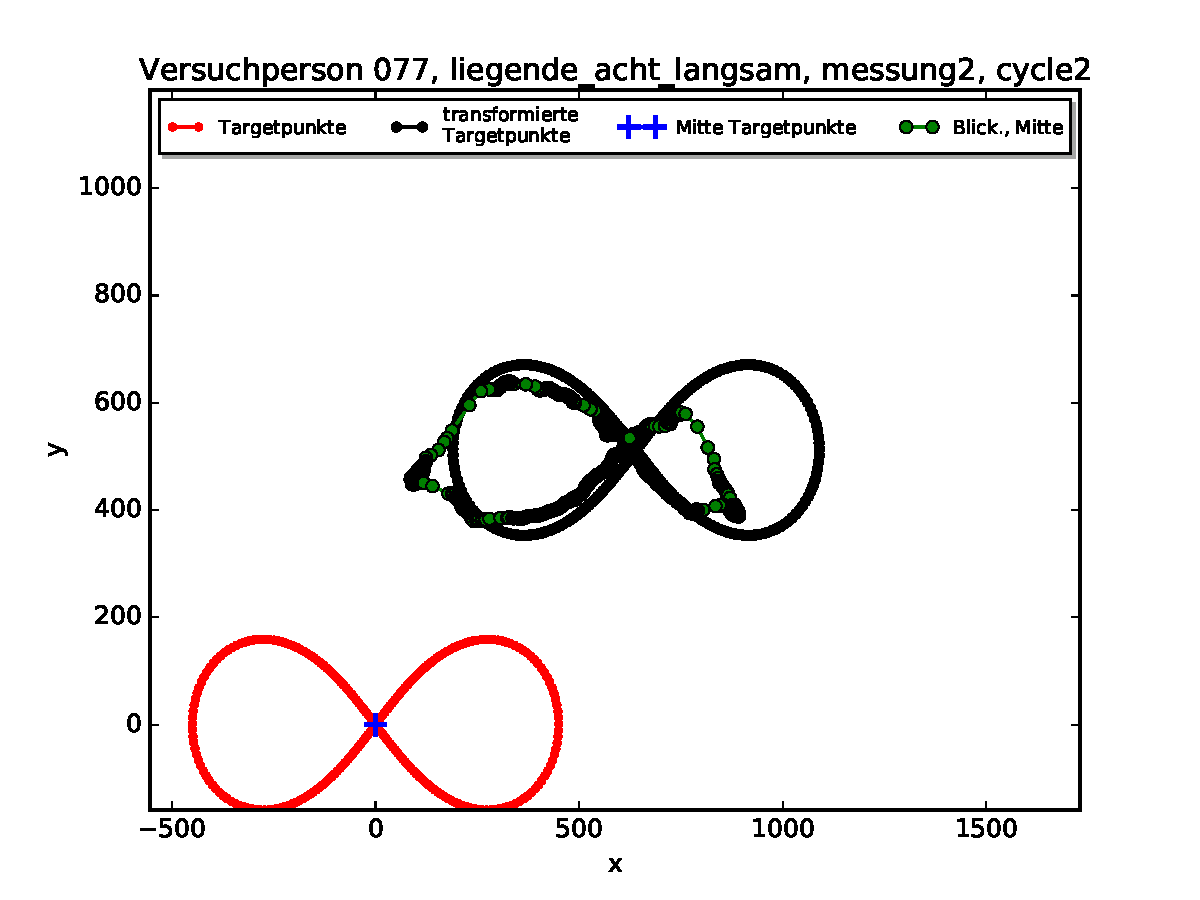
\includegraphics[width=10cm]{Bilder/AufzeichnungVP77.pdf}
		\par\end{centering}
	\caption{\label{fig:rohdaten}Beispiel liegende Acht von Versuchsperson 77: in rot sind die aufgezeichneten Zielpunkte zu sehen, in gr\"un die Mittleren Blickpositionen. In schwarz sind die transponierten Targetpunkte dargestellt.}
    \end{minipage}
	\qquad
    \begin{minipage}[ht]{10cm}	
	\noindent \begin{centering}
		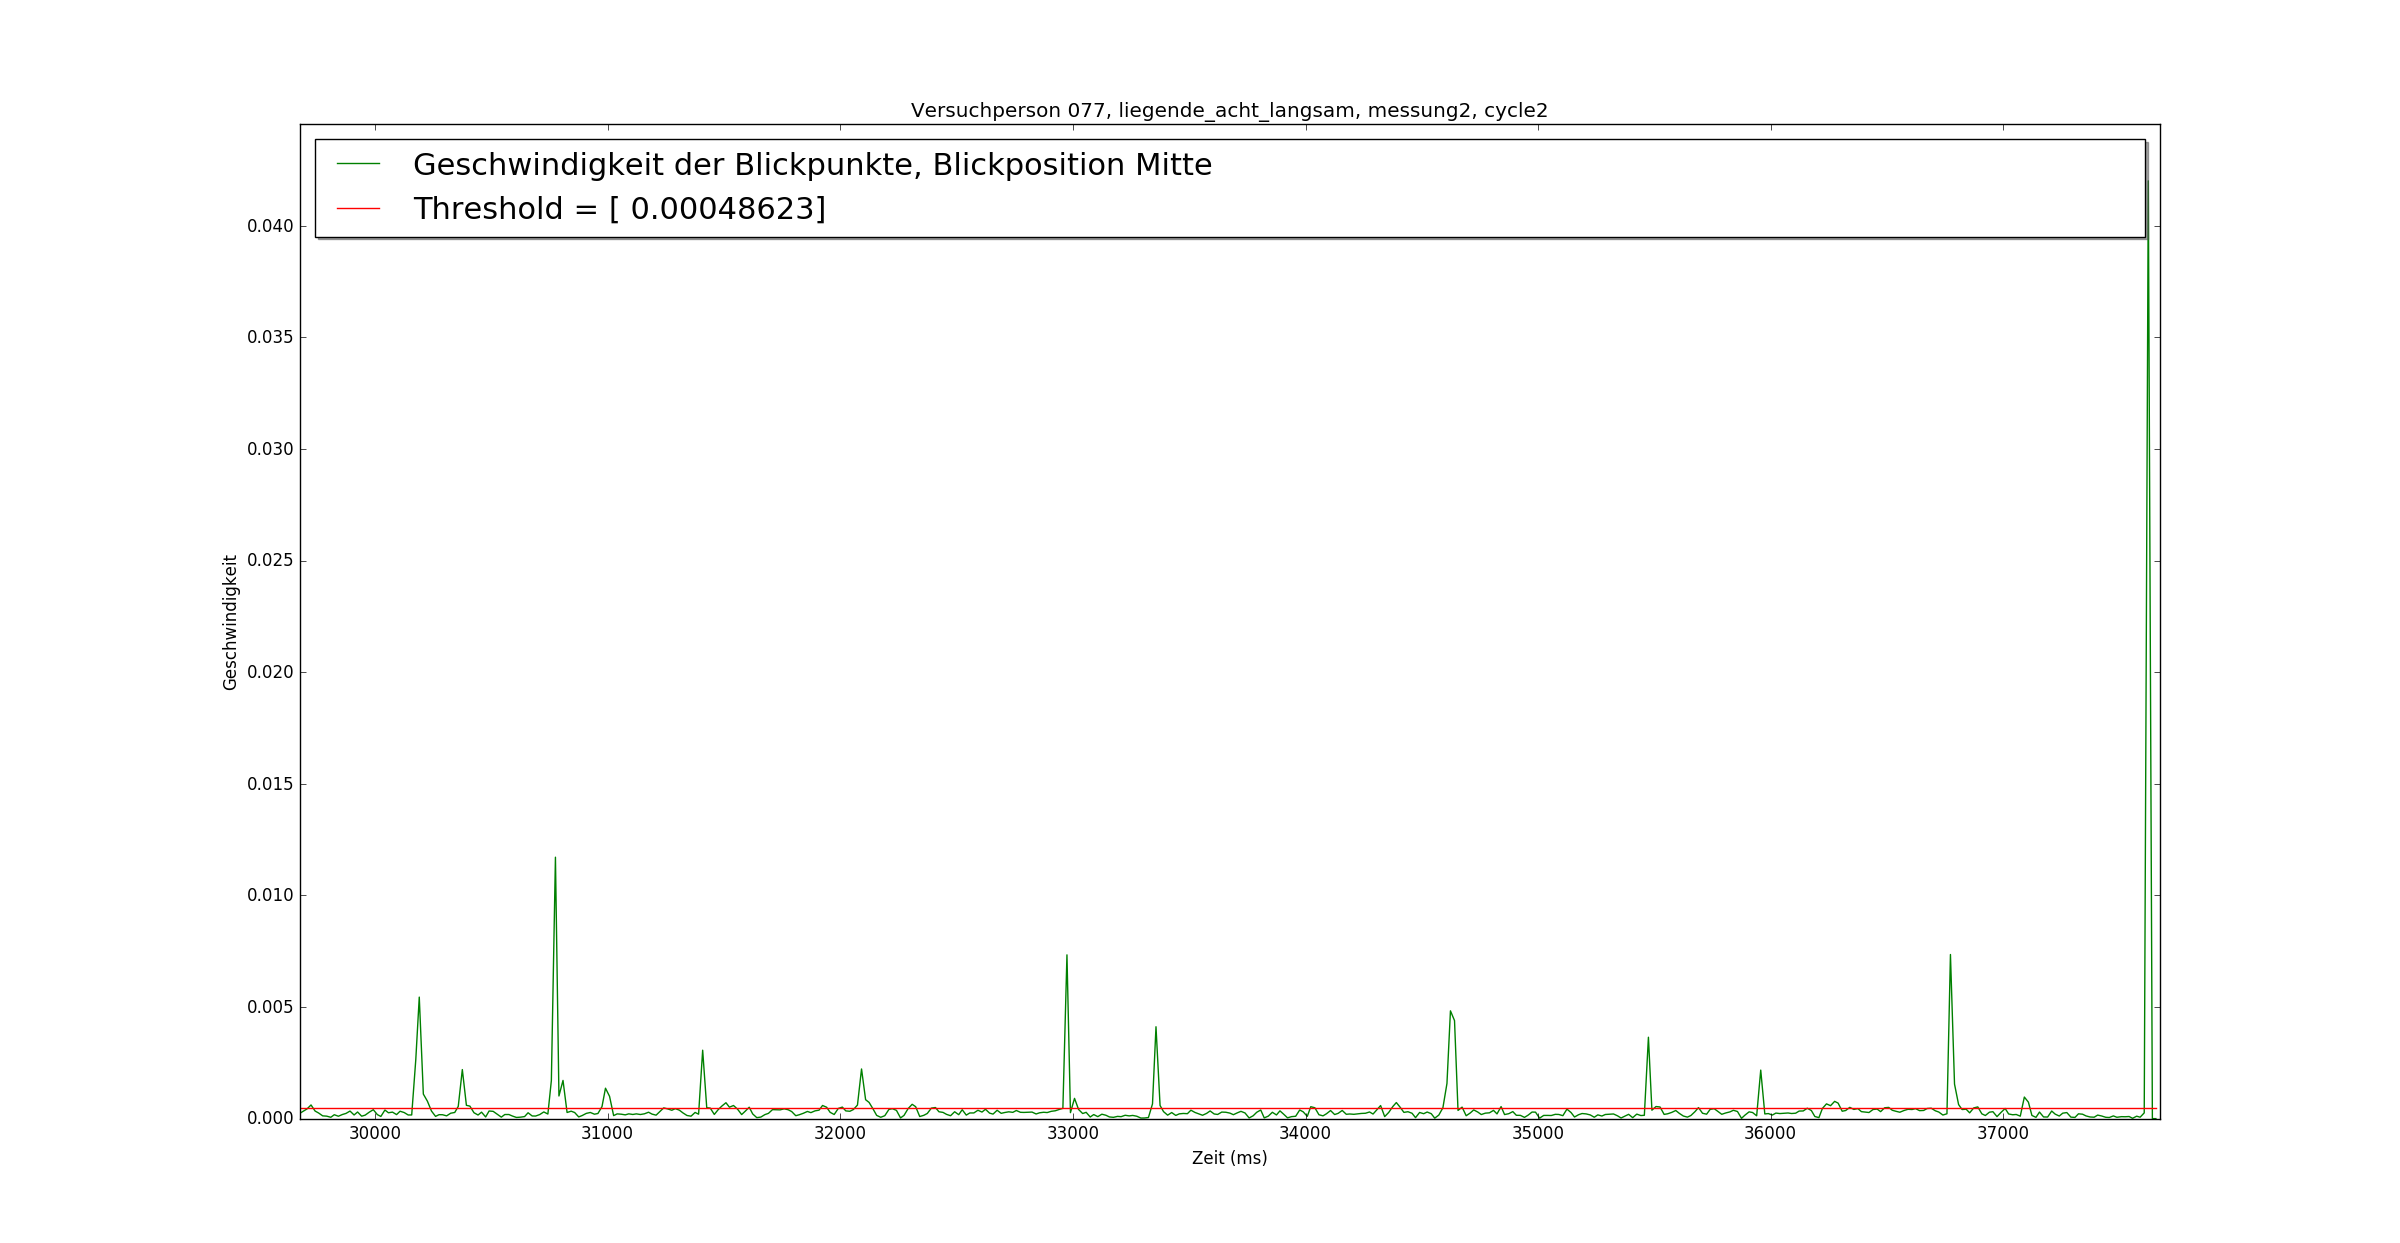
\includegraphics[width=10cm]{Bilder/figure_saccade_vp_77.png}
		\par\end{centering}
	\caption{\label{fig:DiagrammSakkaden}Beispiel Versuchsperson 77: Die rote Linie ist der Schwellwert, f\"ur die Geschwindigkeit, damit eine Augenbewegung als Sakkade gez\"ahlt wird. Die gr\"une Kurve ist der Verlauf der mittleren Augenposition zwischen linken und rechten Augen w\"ahrend eines Versuchs liegende Acht.}
    \end{minipage}
\end{figure}
\end{landscape}

\bibliography{quellen}

\bibliographystyle{alphadin}

\end{document}